\chapter{Discussion}
\label{cha:discussion}

In Chapters \ref{cha:bayespc}-\ref{cha:lida} above, we have argued for the necessity of probabilistic mechanisms in spatial cognition when faced with a complex, uncertain environment perceived through noisy sensors. Although by no means conclusive, we have presented evidence that

\begin{enumerate}
	\item hippocampal place cells represent spatial uncertainty, 
	\item they can perform approximate Bayesian inference,
	\item the representations by recently active place cells can be corrected near-optimally through reverse replay when revisiting a place, and
	\item spatial representation structure arises from clustering under a metric defined over features including distance and visual and functional similarity.
\end{enumerate}

We have also integrated these suggested probabilistic mechanisms into LIDA, and embodied the resulting cognitive architecture in a robotic simulation. In this Chapter we first briefly outline our tentative neural model of these same mechanisms (Figure \ref{fig:neurimpl}). Subsequently, we discuss the abilities, shortcomings, and missing functionalities of our models, and their consistency with related empirical findings, from a cognitive science perspective. 

\nocite{deshmukh2013}

\begin{figure}[h]
	\centering
	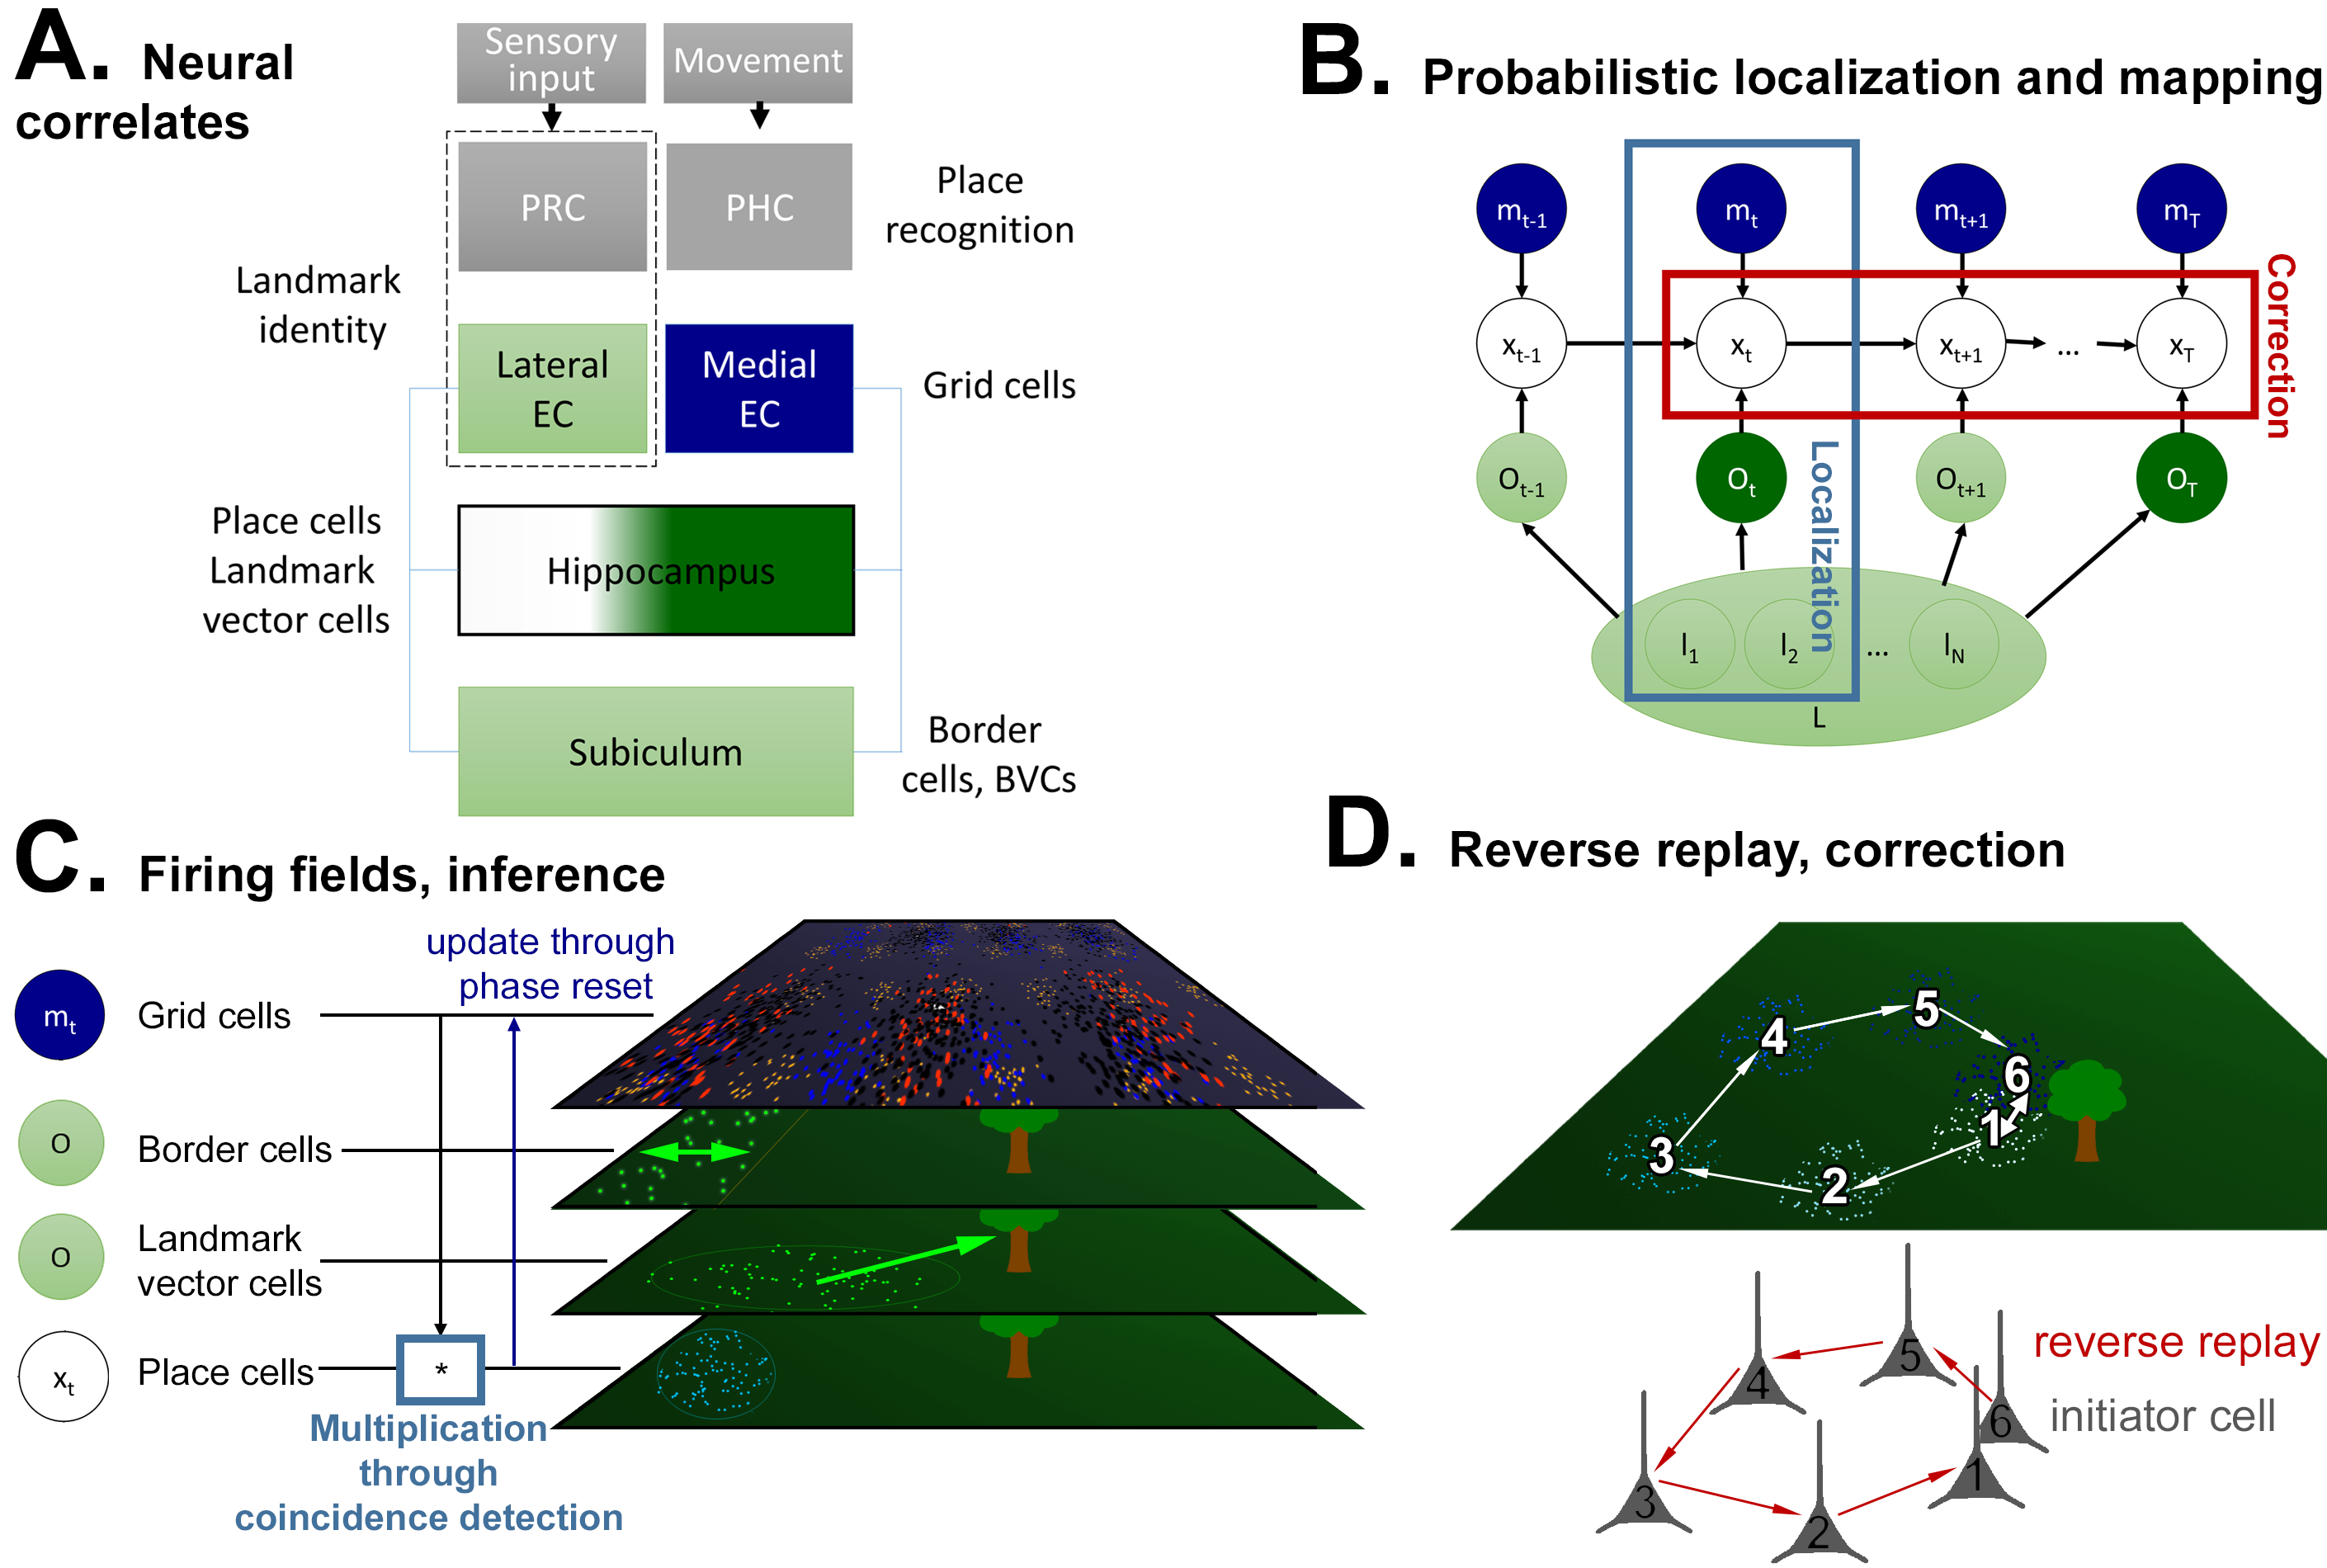
\includegraphics[width=\textwidth]{img/neurimpl3}
	\caption[Probabilistic spatial localization and mapping on the neuronal level]{\textbf{Probabilistic spatial localization and mapping on the neuronal level}. A: Neural correlates of localization (see Chapter \ref{cha:nnreview} for details; and (Deshmukh et al., 2013) for evidence of landmark vector cells). B: Probabilistic graphical model of the simultaneous localization and mapping problem \citep{thrun2008simultaneous}. Instead of capturing all correlations introduced through the landmarks, which requires vast computational resources, our model separately solves Bayesian localization with only local landmarks, and map correction (`pose optimization' in SLAM) with only loop closure constraints. See Chapter \ref{cha:methods} for notation and details. C: Illustration of firing fields during localization. Coloured dots represent spikes of the respective cells at specific locations. Path integration (grid cells) and boundary and landmark information (border cells, landmark vector cells) is integrated in place cells, using coincidence detection (rejection sampling) to obtain a near-optimal location estimate. This new estimate is used to update grid cell representations via phase reset to combat accumulating path integration errors (see Chapter \ref{cha:bayespc}). D: Illustration of a small loop (firing fields 1-6) which can be corrected upon recognizing the same landmark at positions 1 and 6 via reverse replay, by reactivating place cells 6-1 and shifting their place fields proportionally (see Chapter \ref{cha:lida}).} 
	\label{fig:neurimpl}
\end{figure}

%\section{A neural model of Bayesian mechanisms in spatial cognition}

\section{Other mechanisms and representations involved in spatial navigation}

%Naturally, explaining some amount of variance in a handful of datasets is not sufficient to validate a cognitive model. Ideally, a broad range of behaviour data from different tasks should be explainable using the same model with the same parameters, which is the ultimate goal of the LIDA cognitive architecture \citep{franklin2013lida} - but such extensive validation is beyond the scope of the current work. In this work, we have merely aimed to maximize consistency with established findings related to spatial cognition, implementability within known neural structures, and fit empirical data. The result chapters above have mostly focused on the latter. In this Chapter, we will briefly discuss the former two.

Tables \ref{tbl:spmech} and \ref{tbl:sprep} summarize the processes and representations involved in spatial navigation in biological cognition. The first columns provide overviews of these mechanisms and representations, based on Figure 1 in \citep{wolbers2010determines}. The second column indicates the corresponding mechanism in our final LIDA-based model, as described in Chapter \ref{cha:lida}. The rightmost column highlights some major elements missing from the models presented here but required for spatial navigation. 

%\begin{tabular}[c]{@{}c@{}} a \\ b \end{tabular}

\begin{table*}[h]
	\centering
	{ %\renewcommand{\arraystretch}{1.2}
		\begin{tabu}{c|c|c}
			$\downarrow$ {\textbf{Mechanism}} & {\textbf{In our model}} & {\textbf{Not implemented}} \\ \tabucline[3pt]{-}
			\multicolumn{3}{c}{\textbf{Spatial computations}} \\ \hline
			Space perception & \begin{tabular}[c]{@{}c@{}} Limited (depth from \\ stereo disparity*) \end{tabular} & \begin{tabular}[c]{@{}c@{}} Estimating size, shape, \\ movement, orientation, ... \end{tabular} \\ \hline
			Self-motion perception & \begin{tabular}[c]{@{}c@{}} Surrogate: odometry* \end{tabular} & \begin{tabular}[c]{@{}c@{}} Motor efference, proprio- \\ ceptive \& vestibular senses \end{tabular} \\ \hline
			\begin{tabular}[c]{@{}c@{}} Translation btw. ego- and \\ allocentric reference frames \end{tabular} & \begin{tabular}[c]{@{}c@{}} Limited: Perspective \\projection via \\homography* \end{tabular} & \begin{tabular}[c]{@{}c@{}} Plausible translation \\ mechanism \end{tabular} \\ \hline
			\begin{tabular}[c]{@{}c@{}} Computing directions and \\ distances to unseen goals \end{tabular} & \begin{tabular}[c]{@{}c@{}} Route plan SBC \\ (following gradient \\ on a hierarchical grid) \end{tabular} & \begin{tabular}[c]{@{}c@{}} Explicit direction \\ estimation, systematic \\ errors in estimation \end{tabular} \\ \hline
			\begin{tabular}[c]{@{}c@{}} Imagining shifts in \\ spatial perspective \end{tabular} & - & Sensory imagery \\ \hline
			
			\multicolumn{3}{c}{\textbf{Executive processes}} \\ \hline
			Novelty detection & - & \begin{tabular}[c]{@{}c@{}} Perceptual recognition of \\ known or novel places \end{tabular} \\ \hline
			\begin{tabular}[c]{@{}c@{}} Selection and maintenance \\ of navigational goals \end{tabular} & \begin{tabular}[c]{@{}c@{}} Attention codelets* \\ \& global broadcast* in \\ LIDA's cognitive cycle \end{tabular} & \begin{tabular}[c]{@{}c@{}} Reward representations, \\ reinforcement learning \end{tabular} \\ \hline
			Route planning or selection & \begin{tabular}[c]{@{}c@{}} Route plan SBC \\ (following gradient \\ on a hierarchical grid) \end{tabular} & \begin{tabular}[c]{@{}c@{}} Expectation violation / \\ confirmation monitoring, \\ re-planning, homing...\end{tabular} \\ \hline
			\begin{tabular}[c]{@{}c@{}} Uncertainty/Conflict \\ resolution \end{tabular} & \begin{tabular}[c]{@{}c@{}} Partial: Bayesian \\ integration \end{tabular} & \begin{tabular}[c]{@{}c@{}} Conflicting cues, \\ cues other than odometry \\ \& estimated distance  \end{tabular} \\ \hline
			Resetting mechanisms & \begin{tabular}[c]{@{}c@{}} Partial: maximum \\ likelihood correction \end{tabular} & \begin{tabular}[c]{@{}c@{}} Kidnapped robot \\ problem \end{tabular} \\ \hline
		\end{tabu}
	}
	\caption[Cognitive mechanisms involved in spatial navigation]{\textbf{Cognitive mechanisms involved in spatial navigation}, based on \citep{wolbers2010determines}. *: an ability of our model making use of existing implementations (in the LIDA cognitive architecture or the Robot Operating System).}
	\label{tbl:spmech}
\end{table*}

\clearpage

\begin{table*}[h]
	\centering
	{ %\renewcommand{\arraystretch}{1.2}
		\begin{tabu}{c|c|c}
			$\downarrow$ {\textbf{Representation}} & {\textbf{In our model}} & {\textbf{Not implemented}} \\ \tabucline[3pt]{-}
			\multicolumn{3}{c}{\textbf{Online representations}} \\ \hline
			Self-position and orientation & `Self' PAM node & - \\ \hline
			\begin{tabular}[c]{@{}c@{}} Egocentric self-to-object \\ directions and distances \end{tabular} & \begin{tabular}[c]{@{}c@{}} Limited (depth from \\ stereo disparity*) \end{tabular} & \begin{tabular}[c]{@{}c@{}} Egocentric vectors (e.g. \\ `reach vectors' in area 5a) \end{tabular} \\ \hline
			\begin{tabular}[c]{@{}c@{}} Allocentric object-to-object \\ directions and distances \end{tabular} & \begin{tabular}[c]{@{}c@{}} Indirect (on map \\ representation, but not \\ perceptually) \end{tabular} & \begin{tabular}[c]{@{}c@{}} Allocentric visuo- \\ spatial representations \end{tabular} \\\hline
			Route progression & `Route' PAM nodes & Expectations \\\hline
			Navigation goals & `Goal' PAM nodes & Rewards \\\hline
			\multicolumn{3}{c}{\textbf{Offline representations}} \\ \hline
			\begin{tabular}[c]{@{}c@{}} Memories of local \\ views and places \end{tabular} & \begin{tabular}[c]{@{}c@{}} Partial (in pre-conscious \\ working memory, not \\yet in long-term memory) \end{tabular} & \begin{tabular}[c]{@{}c@{}} Long-term memory \\ representations \end{tabular} \\\hline
			\begin{tabular}[c]{@{}c@{}} Enduring, hierarchical \\ representations of an \\ environment (ego-/allocentric) \end{tabular} & \begin{tabular}[c]{@{}c@{}} Hierarchical maps \\ consisting of \\ `place nodes' \end{tabular} & \begin{tabular}[c]{@{}c@{}} Hierarchical egocentric \\ representations \end{tabular} \\\hline
			Networks of habitual routes & \begin{tabular}[c]{@{}c@{}} Context-action-result chains \\ in Procedural Memory* \end{tabular} & - \\\hline
		\end{tabu}
	}
	\caption[Representations involved in spatial navigation]{\textbf{Representations involved in spatial navigation}, based on \citep{wolbers2010determines}}
	\label{tbl:sprep}
\end{table*}


\section{Limitations and shortcomings}

In addition to mechanisms and representations playing an important role in spatial navigation but not yet implemented in our model (Tables \ref{tbl:spmech} and \ref{tbl:sprep}), there are several shortcomings of our models, which we outline in this Section. They can roughly be grouped into three categories: computational shortcomings, psychological implausibilities, and neural implausibilities.

\subsection{Computational shortcomings}

We have pointed out in Chapters \ref{cha:intro} and \ref{cha:methods} that the goal of this work was not to optimize for performance (but rather computational cognitive modelling), and that these problems can be solved more optimally and accurately, given enough computational resources. Accuracy and performance of spatial representations are the goals of Simultaneous Localization and Mapping (SLAM) in mobile robotics \citep{thrun2008simultaneous}. 

State of the art solutions to the SLAM problem can infer robot and landmark locations down to a few centimetres accuracy or better, but usually require $5-25 \%$ of the processing power of a current Intel Core i7-3630QM CPU to do so \citep{machado2013evaluation}, even when just mapping a small room, which amounts to $4-20$ billion floating point operations per second\footnote{Based on Intel i7 specifications, retrieved from  \url{http://download.intel.com/support/processors/corei7/sb/core_i7-3600_m.pdf}}. Achieving the same in large-scale outdoor environments would require even more computational resources.

Figure \ref{fig:endtoendslam} shows the structure of modern end-to-end SLAM systems \citep{wang2015}, such as e.g. \citep{newman2011describing}. Components depending on the specific sensors and actuators ('front-end') are usually separated from the sensor-independent optimization part (`back-end'). In our final model described in Chapter \ref{cha:lida}, the `front-end' roughly corresponds to the functionality of the Bayesian localization SBC, and the `back-end' to that of the Map correction SBC. Both functionally correspond to hippocampal place cells, with the former mechanism implemented by coincidence detection, and the latter through reverse replay. 

\begin{figure}[h]
	\centering
	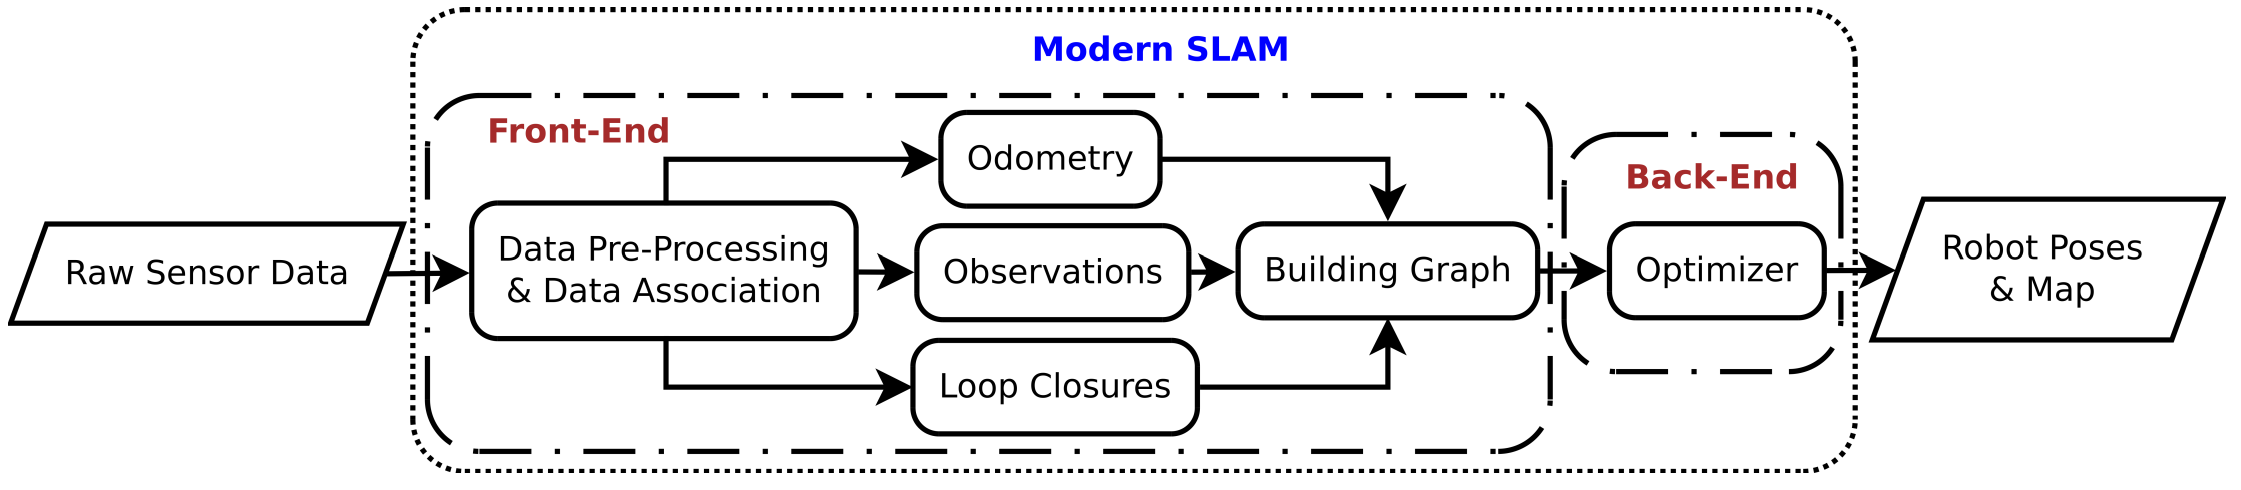
\includegraphics[width=\textwidth]{img/endtoendslam}
	\caption[Components of a modern end-to-end SLAM system]{\textbf{Components of a modern end-to-end SLAM system}. From \citep{wang2015}} 
	\label{fig:endtoendslam}
\end{figure}

The two main computational shortcomings compared to modern SLAM include 1) not explicitly modelling rotations (thus avoiding non-linearity caused by robots which can turn), and 2) not explicitly optimizing landmark constraints (only path integration and loop closure constraints). These cause inferior localization and mapping accuracy compared to modern SLAM. However, they have allowed us to map Bayesian mechanisms to well-known neural correlates and mechanisms, and to implement simple models successfully replicating behaviour data, while still retaining the ability to tackle the uncertainty and noise problem in a realistic robotic simulation.

Although brains may well be capable of the processing power required by a SLAM system, it is unlikely that they work the way modern SLAM solutions do (performing thousands of linear algebra operations serially) \citep{thrun2008simultaneous}. Furthermore, human long-term memories are far from being as accurate as these SLAM systems, as shown e.g. in Figures \ref{fig:lida:nardini} and \ref{fig:lida:comparison} in Chapter \ref{cha:lida}, or by research regarding sketch maps, e.g. \citep{rovine1989sketch, wang2009accuracy}. Nevertheless, there is value in looking at information processing in brains through the lens of normative models, of mathematical formulations of the problem to be solved; and of their implementability in brains and minds. 

\subsection{Psychological implausibilities}

Apart from implementation details (in brains and in LIDA), on Marr's (1976) algorithmic level, three mechanisms were suggested in this thesis: 1) a cue integration mechanism for localization, 2) correction of cognitive maps when re-visiting places, and 3) cognitive map structuring through clustering. Despite of their ability to fit behaviour data as described in Chapters \ref{cha:bayespc}-\ref{cha:lida}, there are some psychological findings which are inconsistent with these mechanisms. 

First, our models have focused on adult cognition, and have ignored developmental findings. Visual spatial integration progressively improves in children between 5 and 14 years of age \citep{kovacs1999late}. Spatial cue integration, while close to the Bayesian optimum in adults, seems to require a long developmental process; and children do not seem to integrate spatial cues, instead switching between exclusively using path integration or landmark information from trial to trial \citep{nardini2008development}. It is difficult to model this behaviour in our Bayesian framework.

In terms of adult spatial cognition, there are shortcomings in how landmarks are recognized. In the current model, any objects recognized by the CNN briefly described in \ref{cha:lida} constitutes a landmark. However, in human (and animal) cognition, landmarks have to be reliable, salient, stable (unmoving), and possibly distal \citep{lew2011looking}. These criteria defining landmarks for biological spatial cognition are not accounted for in the model. Neither are cues in the form of landmark arrays (e.g. humans use the natural axes of regular arrays of objects as a reference frame) \citep{lew2011looking, burgess2006spatial}. 

Phenomena observed in environments with competing cues (e.g. landmarks), where the information from the cues is not integrated, are also difficult to model in our probabilistic framework. Examples include `overshadowing' (where the effect of a cue on an animal's behaviour may be reduced or eliminated when another, more salient cue is introduced) and `blocking' (where a second cue is added after an animal has been trained with the first, but the animal cannot use the second cue without the first) \citep{chamizo2003acquisition}. Some evidence of landmark overshadowing and blocking in humans exists, e.g. \citep{spetch1995overshadowing, prados2011blocking}, and it has been argued that unlike the role of boundaries, associative reinforcement (and not a map-like representation) may be a better explanation for landmark learning \citep{doeller2008distinct}. 

Navigation based on two complementary systems running in parallel (a cognitive mapping system using the described mechanisms, and a reward-based associative learning system based on LIDA's procedural memory) is conceptually consistent with blocking and overshadowing, and may be able to explain these findings. We have not implemented this computationally, however; and the extent of cooperation / competition between these systems is not yet clear, even on a theoretical level \citep{lew2011looking, cheng201325}.

In addition to the role of landmarks, a `geometric module' for navigation has been proposed, originally to explain errors which would have been avoidable if perceptual as opposed to geometric cues had been used (such as rats learning there is food in the corner of a rectangular environment, but often searching in the diagonally opposite corner of the environment, which was geometrically - but not perceptually - equivalent) \citep{cheng1986purely}. Similar geometry-based behaviour has been observed in young children, e.g. by \cite{huttenlocher1999spatial} (see also \citep{cheng201325}). Recent findings cast the existence of a dedicated geometric module for orientation and navigation in doubt \citep{cheng2008whither}. Nevertheless, empirical observations of such errors (which are consistent with geometry-based orientation, but could be avoided by making use of perceptual features/landmarks) are inconsistent with our model, which does not make such errors.

Other types of systematic errors in spatial representations have been pointed out in the literature which our model does not account for in its current form. Distortions result from the hierarchical organization in cognitive maps \citep{tversky1992distortions,hirtle1985evidence} - which, however, could easily be incorporated into the model, given that it already learns these hierarchies (all that is required is implementing an error function/mechanism). However, there are also systematic distortions of spatial representations which are not easily accounted for in this framework. They include effects of perspective (where participants are asked to imagine themselves when asked to estimate spatial relations), of cognitive reference points (distance judgements made from landmark A to building B usually differ from those made from building B to landmark A), and of detours or barriers (the length of circuitous routes is usually overestimated) - see \citep{tversky1992distortions, tversky2003navigating}. Differences in viewpoints used when learning spatial representations and when having to use them also cause systematic errors (e.g. \citep{shelton2001systems, Shelton2004, burgess2006spatial}) which have been neglected by the current models.

Finally, the current model, when forced to explore very large regions without being allowed to ever revisit known places, can incur catastrophically large errors to its learned representations, making the learned map largely useless (we know of no such effect observed in humans). It is likely that in very large scale environments, humans make use of several parallel mechanisms including spatial reasoning, as well as of prior knowledge of the structure of the environment (e.g. the usual shapes of roads), none of which have been included in the model. 

We note that to our knowledge, no current computational cognitive model of spatial memory achieves full consistency with every empirical finding, while being capable of running in realistic environments at the same time (see review in Chapter \ref{cha:nnreview}). We have argued that our approach is a step in the direction of such models, which can be the case even if it does not support modelling some known aspects of spatial cognition. As long as the basic premises hold (that brains can represent uncertainty, and can perform approximate Bayesian inference), and if the shortcomings can be corrected in future models in a cognitively plausible fashion, the probabilistic approach to spatial cognition remains viable.


\subsection{Neural implausibilities}

In terms of consistency with neuroscientific findings, we have to distinguish between the final computational cognitive model based on the LIDA cognitive architecture (Chapter \ref{cha:lida}), and the suggested neural mechanisms regarding uncertainty representation and error correction in the hippocampus. We omit discussing the neural plausibility of the map structuring model introduced in Chapter \ref{cha:nnreview}, since we have not described any neural implementation of this mechanism, and only validated it behaviourally (but see e.g. \citep{shi2009neural} or \citep{sanborn2015types} for possible neural implementations of hierarchical Bayesian models, to which the DP-GMM belongs). It is to our knowledge the first model able to predict spatial representation structure on the individual level; and developing a biologically plausible implementation in addition to a normative and algorithmic model would have exceeded the time available for this PhD.

Regarding the final model (Chapter \ref{cha:lida}), LIDA intends to be a model of minds, not brains (it is a model on Marr's algorithmic and not implementation level) - see \citep{franklin2012global, franklin2013lida} for discussions of the relationship between LIDA and the underlying neuroscience. Nevertheless, we briefly point out a few mechanisms of the model in Chapter \ref{cha:lida} (LIDA extended by the described probabilistic spatial mechanisms and embodied on a robot) which do not directly correspond to known neural processes. 

The first salient difference is the visual recognition system, for which we used existing implementations to make this work tractable within one PhD. Specifically, we used convolutional neural networks for recognizing objects \citep{szegedy2014going} and roads \citep{brust2015convolutional}, which have been designed for maximizing recognition performance, not for neural plausibility. Curiously, they do seem to learn representations that are very similar to those recorded in human and primate inferior temporal cortex \citep{khaligh2014deep, yamins2013hierarchical}. But their conventional training algorithms are not implementable in biological neurons \citep{stork1989backpropagation, bengio2015towards}. Developing a plausible recognition system would have exceeded the scope of this PhD. The same is true for motor control, for which we used existing drivers of the Robot Operating System\footnote{See \url{http://wiki.ros.org/pid} and \url{http://gazebosim.org/tutorials?tut=drcsim_fakewalking&cat=drcsim}} (which are by no means brain-like).

In terms of the spatial extensions to LIDA, the biggest discrepancy is the regular grid formed by the `place nodes' (Chapter \ref{cha:lida}). Place cells do not seem to map the surface of an environment in any systematic fashion \citep{o1998place}. It would be more accurate to think of `place nodes' as combining several underlying spatially relevant cell types, including entorhinal grid cells, which do form regular grids (although triangular and not rectangular) \citep{moser2008place}. Grid cells also facilitate estimating directions and distances \citep{bush2015using}. However, the simple route planning strategy (based on spreading activation on hierarchical grids of place nodes) is not a faithful model of navigation in the hippocampal entorhinal complex, as it heavily relies on a regular structure and on specific link weights depending on distances and obstacles. \cite{bush2015using} reviews four more biologically plausible network models on Marr's implementation level. However, LIDA is concerned with the algorithmic level - and there is published behavioural evidence for such a mechanism \citep{mueller2013pathfinding}. We have also succeeded in replicating several multi-goal route planning datasets using our simple model (see Appendix \ref{apx:lidaspm}), which substantiates its cognitive plausibility. 

On the other hand, the plausibility of the probabilistic framework for cognitive modelling does require, at the very least, the possibility of neurally implementing Bayesian inference. To show evidence of this possibility, we have compared the firing of hippocampal place cells to predictions of a Bayesian model, and have suggested they might be able to represent uncertainty and perform approximately optimal inference (see Chapter \ref{cha:bayespc}). These are hypotheses on the neuronal level. As such, they can be compared to neuroscientific findings - and they do seem to be inconsistent with some, as summarized below.

First, humans with hippocampal lesions, although spatially impaired, do seem to be capable of spatial navigation. For example, \citep{teng1999} report a patient with damaged medial temporal areas who was able to describe routes, detours, and directions between landmarks in an environment he has learned early, before the damage. The authors suggest that the role of the hippocampus is time-limited, mostly concerning consolidation, and that long-term spatial memories are available after consolidation even with a lesioned hippocampus. Similar observations of largely unimpaired topographical abilities in patients with hippocampal damage were found by \citep{rosenbaum2000, rosenbaum2005}; although these patients did show some types of impairments (few recalled landmarks on sketch maps, no detailed geographical knowledge, impaired landmark recognition). A later study by \cite{maguire2006} reinforced the implication that although accessing long-established spatial memories is still possible with a damaged hippocampus, topographical knowledge of landmarks and of the relationships between them is impaired. Naturally, the ability to learn new spatial representations is also heavily impaired. Nevertheless, some functionalities requiring allocentric representations seem to be available to patients with hippocampal lesions, which is problematic for the `cognitive map' hypothesis in general, as well as for our model.

Second, the firing fields of place cells do not behave like unique, one-to-one representations of location. Some place cells (a minority) have more than one firing field \citep{burke2011influence}, and there do not seem to be systematic commonalities between these (e.g. similar distances to surroundings) as would be predicted by a model using these firing fields as probability distributions. Place fields are also not always regular and elliptic, as prescribed by the simplest Gaussian model in Chapter \ref{cha:bayespc} (although this is not an issue for the particle filter-based formulation in Chapter \ref{cha:lida}, which can represent multimodal distributions). Furthermore, it is not the case that place fields close to boundaries are always smaller than those further away, as would be predicted if they solely represented uncertainty. For example, firing fields of cells in dorsal hippocampus are generally smaller than those of cells in more ventral areas \citep{kjelstrup2008finite}. Finally, there are several phenomena observed in recordings from place cells of behaving animals which do not easily fit into a probabilistic model. These include remapping \citep{colgin2008understanding} and theta phase precession \citep{skaggs1996theta}.

However, these inconsistencies do not falsify the possibility of an approximate Bayesian inference mechanism operating in the hippocampus in parallel to several other mechanisms not accounted for (and in some cases inconsistent with) such a mechanism. Brains exhibit a high degree of redundancy, and there is no reason to assume that one cell type only performs one function. Over-reliance on only a single or few place cells inconsistent with the statistical optimum could destroy the models functionality. However, a larger ensemble of place cells, a majority of which do represent location estimates and their associated approximate uncertainty, can still facilitate approximately optimal localization if the contradicting information in the ensemble (representing other things, such as an episodic memories \citep{tulving1998episodic}) is a minority. The approximate Bayesian hippocampus hypothesis could be falsified if the number of place cells used for localization, and having firing fields inconsistent with Bayesian uncertainty predictions, could be shown to be a majority. However, this does not seem to be the case in the recordings and environments investigated here (see Chapter \ref{cha:bayespc}).

We can further support the claim of multiple parallel hippocampal mechanisms, one of which may be approximate Bayesian inference, using three observations. First, the reasonably good fit of Bayesian predictions with empirical place field sizes reported in Chapter \ref{cha:bayespc} would be extremely unlikely to occur by chance, given that hundreds of place fields were included in the comparison. Second, our particle filter localization model is largely robust to artificially increasing or decreasing the variance of the samples at some places\footnote{In fact, adding random samples, independently from the Bayesian prediction, was one of the early methods used in robotics to combat `particle depletion' and to increase the chances of the robot being able to recover its correct location in particle filter-based SLAM \citep{thrun2005probabilistic}.}, which is a rudimentary way of simulating some place fields having a different size than prescribed by a Bayesian model. Finally, the uncertainties predicted by a sampling-based localization model can also successfully explain the frequency distribution of place field sizes (see comparison in Appendix \ref{apx:pfev}). The small amount of deviation between the frequency distribution of uncertainties in the model, and between the frequency distribution of place field sizes, suggests that place fields inconsistent with Bayesian uncertainty were a small minority in this environment. 

%\subsection{Neural implausibilities of approximately Bayesian place cells}

% # PF

% REMAPPING

% getting Sigma is slow

% map correction - explicit distance

% hc power / activity ~ mvmnt speed

%\subsection{Neural implausibilities of map correction by reverse replay}

% map correction - explicit distance


%\section{Alternative explanations}

% Gigerenzer line of work, heuristics instead of approximate optimality - see eg Sanborn 2015

% Barrera, RatSLAM


% what does all this mean? interpret, evaluate

% strengths
% limitations



% neural implementations

% point out that evidence for GC updating has since been found

% caveats, problems, limitations

%Is there agreement or disagreement with previous work?
	% have to properly discuss BVC model (see Hartley slides)
	
%Interpret results in terms of background laid out in the introduction - what is the relationship of the present results to the original question?
%What is the implication of the present results for other unanswered questions

% There are usually several possible explanations for results. Be careful to consider all of these rather than simply pushing your favorite one

%What are the things we now know or understand that we didn't know or understand before the present work?

% What is the significance of the present results: why should we care? 

% This section should be rich in references to similar work and background needed to interpret results.


%-------

% examiners are looking for (In Discussion AND conclusions:)
%- Is the candidate aware of possible limits to confidence/ reliability/validity of the work?
%- Have the main points to emerge from the results been picked up for discussion?
%- Are there links made to the literature?
%- Is there evidence of attempts at theory building or reconceptualisation of problems?Are there speculations?/re they well grounded in the results?